\chapter{Results}
Using the algorithm described above one is able to produce a NURBS representation of a structure, that has been optimized with respect to predefined boundary conditions. Examples of initial boundary conditions as well as the resulting optimized structures are presented in \autoref{sec:tests}. Additionally the described topology optimization tool enables a less complicated design workflow from the user's point of view. That workflow is described in \autoref{sec:uex}.
\section{Test Cases}
\label{sec:tests}
\todointernal[inline,author=Benni]{Include material saved for each!}
\subsection{Cantilever}
\begin{figure}[H]
\begin{center}
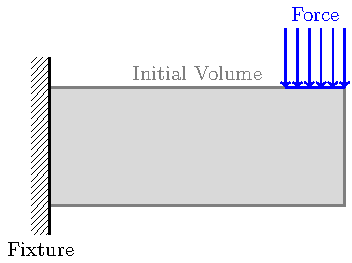
\includegraphics[scale=1]{Pictures/tikzCantilever/canti.pdf}
\end{center}
\caption{Boundary conditions for the test case "Cantilever"}
\end{figure}

\subsection{Bridge}
\begin{figure}[H]
\begin{center}
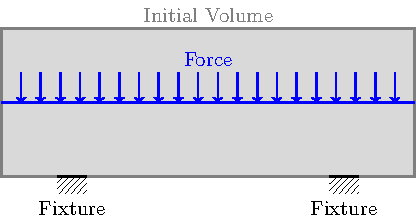
\includegraphics[scale=1]{Pictures/tikzBridge/bridge.pdf}
\end{center}
\caption{Boundary conditions for the test case "Bridge"}
\end{figure}

\subsection{GE Jet Engine Bracket}
\begin{figure}[H]
\begin{center}
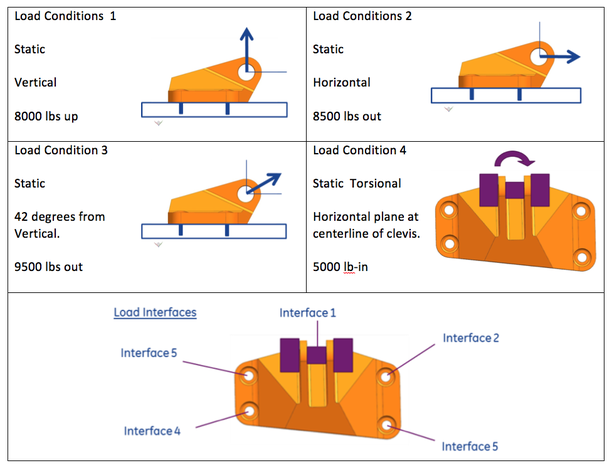
\includegraphics[width=\textwidth]{Pictures/GEbracket.png}
\end{center}
\caption{Boundary conditions and different load cases for test case "GE Bracket". Figure from \cite{GEBracket}}
\end{figure}
Used already optimized design \cite{GEBracketTripon}.


\begin{figure}
\begin{center}
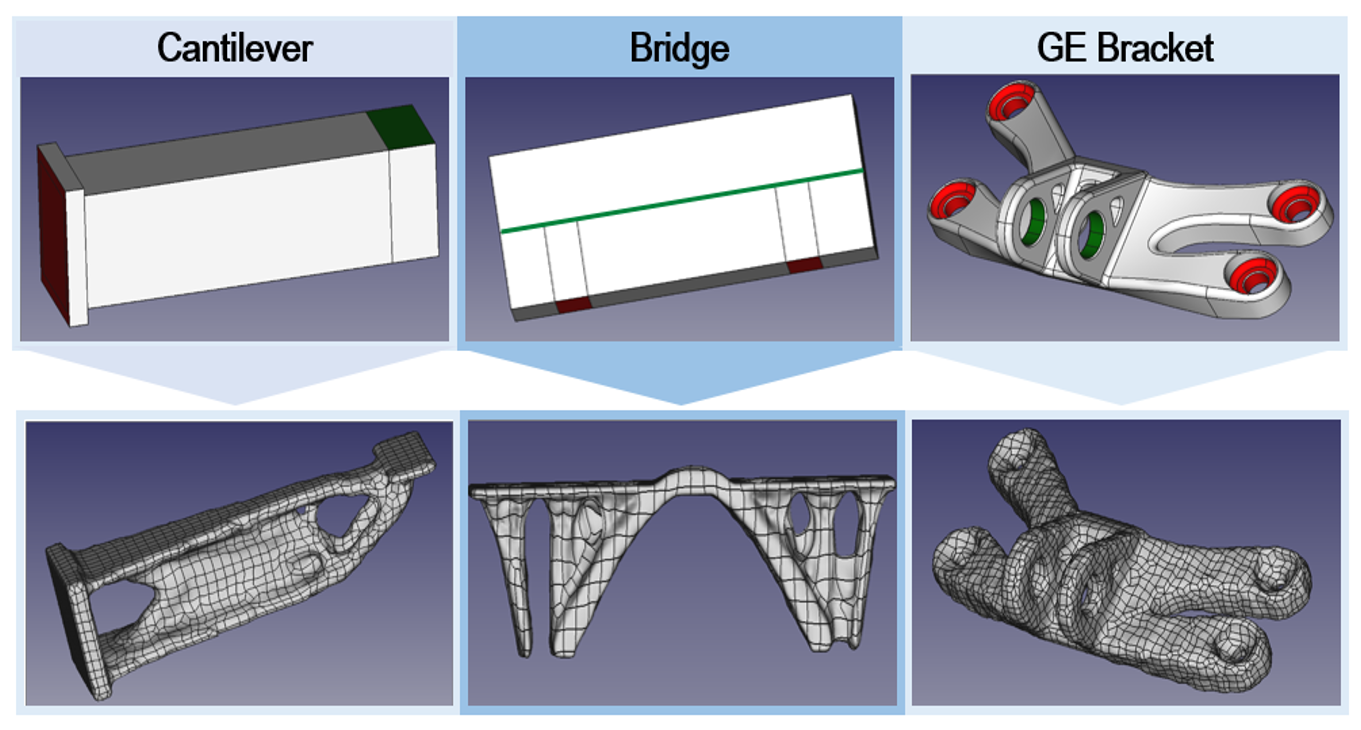
\includegraphics[width = \textwidth]{Pictures/TestCases.png}
\end{center}
\caption{Initial CAD geometry and resulting optimized NURBS geometry for three test cases}
\end{figure}

\section{User Experience}
\label{sec:uex}
From the user point of view CADO  is very simple. One doesn't have to know anything about the algorithms behind nor about the implementation details. Graphical User Interface (see fig. \ref{}) allows the user to enter all the necessary information right a way, without opening the command line and keeping in mind the order of the parameters or the name of the executable file. Closed structure of the pipeline allows us to hide all the technical details from the user. However, user can still see on which stage the process is right now by looking at the progress bars, corresponding to the three major steps:
\begin{itemize}
\item Voxelization
\item Topology Optimimzation
\item Surface Fitting
\end{itemize}

Further information and the detailed description of the user interface can be found in \textit{CADO\_UserGude.pdf}

\todointern{And a nice picture of the GUI from Friedis computer!}
